














\formatChapter{Quartzville Creek}



\raggedcolumns
\begin{multicols}{2}



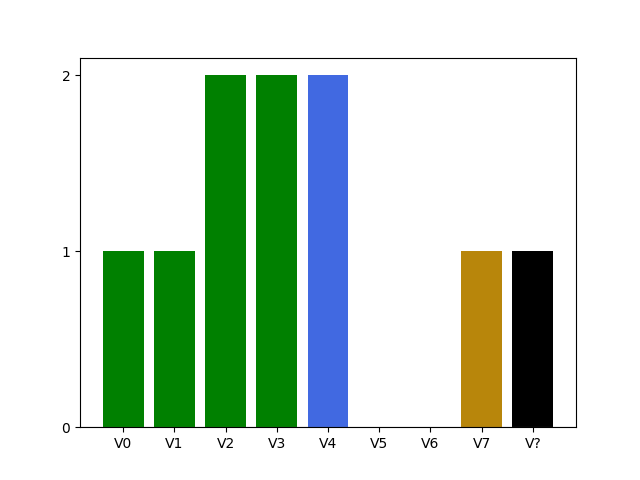
\includegraphics[width=0.9\linewidth]{./maps/plots//Quartzville Creek.png}
\end{multicols}
\begin{multicols}{2}
About an hour further down the road from the main area there are a few interesting boulders in a creek. Generally lower temperatures, free camping, and pleasant swimming holes make this a nice mid summer spot.\\

\textbf{NOTE: This area is mostly incomplete. Look forward to more information in future revisions of this book or contribute your own knowledge on github.}\\


\newpage
	\setbox0=\hbox{\begin{overpic}[width=0.8\linewidth]{./maps/area/redneck_c.png}
	\end{overpic}}
	\needspace{\ht0}
	\begin{center}
	\begin{overpic}[width=0.9\linewidth]{./maps/area/redneck_c.png}
	\end{overpic}
	\end{center}
\label{sm:Redneck Riviera area map}

\section{A - Redneck Riviera}\label{sa:Redneck Riviera}
\qrcode{./maps/qr/Redneck Riviera_qr.png}{http://maps.google.com/maps?q=44.570410945356336,-122.4060701729652}{Navigate to this sub area}
Redneck rivierra is located on Quartzville road apporximately 20.6 miles from highway 20 park in the gravel pull out on the creek side of the road. This is a nice spot with good swimming access and a few established routes on both sides of the river. The locals like to use this spot to pan for gold. In my experience they are friendly and willing to share the space.\\




\needspace{1.5cm}
\subsection*{Pony Boy}\label{bf:Pony Boy}
A small boulder sits on the far bank of the river upriver from the parking.\\
	


\needspace{1.5cm}
\label{rt:Pony Boy}
\colorbox{green!20}{
\parbox{0.95\linewidth}{
\textbf{
1 Pony Boy V2 \ding{73} 
}}}

\begin{adjustwidth}{0.5cm}{}			
Sit start with hands matched in a juggy pocket on the overhanging face of the boulder. Climbing this thing is probably not worth getting your pads wet. (No Topo)
\end{adjustwidth}




\needspace{1.5cm}
\subsection*{Mono Rail}\label{bf:Mono Rail}
Low boulder just below the parking area with an obvious sharp lip that spans the entire downhill face.\\
	


\needspace{1.5cm}
\label{rt:Monorail Project}
\colorbox{black!20}{
\parbox{0.95\linewidth}{
\textbf{
2 Monorail Project V?  
}}}

\begin{adjustwidth}{0.5cm}{}			
Project. Start on the far right and traverse left along the lip. (No Topo)
\end{adjustwidth}




\needspace{1.5cm}
\subsection*{Yo Mamma Boulder}\label{bf:Yo Mamma Boulder}
Yo Mamma is bigger than any of the other boulders in this area. Look for it across the river and downstream from the parking.\\
	


\needspace{1.5cm}
\label{rt:Ugly Face}
\colorbox{green!20}{
\parbox{0.95\linewidth}{
\textbf{
3 Ugly Face V0 \ding{72} \warn
}}}

\begin{adjustwidth}{0.5cm}{}			
Stand start on the left side of the west face of the boulder. This is also the down climb. (No Topo)
\end{adjustwidth}



\needspace{1.5cm}
\label{rt:Binding of Isaac}
\colorbox{green!20}{
\parbox{0.95\linewidth}{
\textbf{
4 Binding of Isaac V2 \ding{72}\ding{72} \warn
}}}

\begin{adjustwidth}{0.5cm}{}			
Stand start with a left hand sidepull about 5ft left of Ugly face. (No Topo)
\end{adjustwidth}




\needspace{1.5cm}
\subsection*{Moss Boss}\label{bf:Moss Boss}
A large mossy boulder on the roadside of the river and downstream of the parking area.\\
	


\needspace{1.5cm}
\label{rt:Moss Boss}
\colorbox{green!20}{
\parbox{0.95\linewidth}{
\textbf{
5 Moss Boss V3 \ding{72} 
}}}

\begin{adjustwidth}{0.5cm}{}			
PLACEHOLDER (No Topo)
\end{adjustwidth}




\needspace{1.5cm}
\subsection*{The 4.5}\label{bf:The 4.5}
A clean overhanging face points downhill the river downstream and across the river from the parking.\\
	


\needspace{1.5cm}
\label{rt:Chicken Tendies}
\colorbox{green!20}{
\parbox{0.95\linewidth}{
\textbf{
6 Chicken Tendies V1 \ding{72} 
}}}

\begin{adjustwidth}{0.5cm}{}			
Stand start with hands matched on a good crimp rail on the left side of the boulder. Climb straight up. (No Topo)
\end{adjustwidth}



\needspace{1.5cm}
\label{rt:Teenage Libertarians}
\colorbox{RoyalBlue!20}{
\parbox{0.95\linewidth}{
\textbf{
7 Teenage Libertarians V4 \ding{72}\ding{72}\ding{72} 
}}}

\begin{adjustwidth}{0.5cm}{}			
Start as for chicken tendies but traverse right and ascend the tallest part of the boulder. (No Topo)
\end{adjustwidth}



\needspace{1.5cm}
\label{rt:Falcon's Reach}
\colorbox{green!20}{
\parbox{0.95\linewidth}{
\textbf{
8 Falcon's Reach V3 \ding{72} 
}}}

\begin{adjustwidth}{0.5cm}{}			
Squat start on a juggy edge. Climb straight up. (No Topo)
\end{adjustwidth}




\newpage

\section{B - Old Miner's Camp}\label{sa:Old Miner's Camp}
\qrcode{./maps/qr/Old Miner's Camp_qr.png}{http://maps.google.com/maps?q=44.58651338802075,-122.35033857932665}{Navigate to this sub area}
Located on Quartzville approximately 24.8 miles from highway 20, the old miner's camp is a popular group campsite there are a few good sized boulders in the river only one boulder has established lines on it. Park either at the camp day use area or on the side of the road immediately above the Dab Rig boulder. Note: the dab rig boulder is typically underwater in the rainy season.\\




\needspace{1.5cm}
\subsection*{The Dab Rig}\label{bf:The Dab Rig}
	


\needspace{1.5cm}
\label{rt:Unsalted Almonds}
\colorbox{Goldenrod!50}{
\parbox{0.95\linewidth}{
\textbf{
1 Unsalted Almonds V7*  
}}}

\begin{adjustwidth}{0.5cm}{}			
PLACEHOLDER (No Topo)
\end{adjustwidth}



\needspace{1.5cm}
\label{rt:Dank Commander}
\colorbox{RoyalBlue!20}{
\parbox{0.95\linewidth}{
\textbf{
2 Dank Commander V4*  
}}}

\begin{adjustwidth}{0.5cm}{}			
PLACEHOLDER (No Topo)
\end{adjustwidth}





\end{multicols}
\clearpage